% ============================================================
%  §1  Introduction
% ============================================================

Vision-language models (VLMs) have improved rapidly, yet adapting a VLM to a new
visual-reasoning task family still typically requires manually curated SFT data or a
hand-designed RL pipeline---per task and per backbone. We ask whether the agent can build
its own task-family-specific capability set instead, by inspecting its own behaviour on a
small training subset and without any weight updates. We illustrate this motivation in
Figure~\ref{fig:motivation}.

\begin{figure}[t]
  \centering
  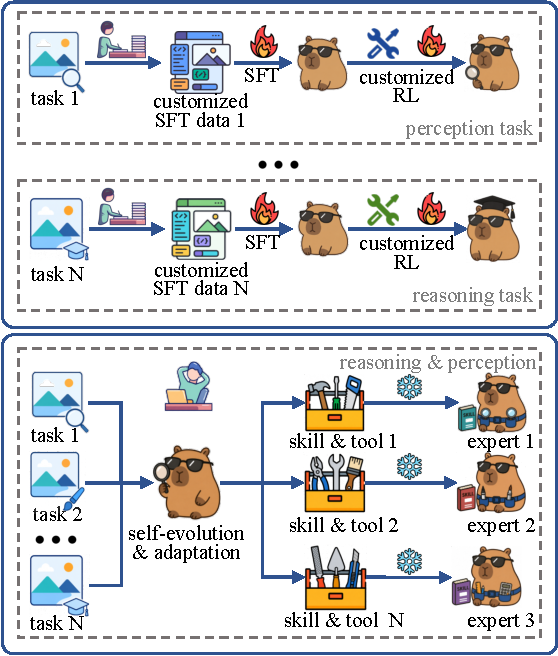
\includegraphics[width=\columnwidth]{figures/Picture2.pdf}
  \caption{
    \textbf{Per-task adaptation without weight updates or hand-authored prompts.}
    Per-task VLM adaptation typically requires manually curated SFT data with a
    hand-designed RL pipeline for every new task family. \sysname{} instead lets a frozen
    VLM agent evolve its own skill and tool set per task family from a small labeled
    training subset---without any weight updates or hand-authored task-specific
    prompts---and dynamically equips the matching set when a case from that family arrives.
  }
  \label{fig:motivation}
\end{figure}

We instantiate this idea in \sysname{}, a training-free framework that evolves two
complementary capability types from a small labeled training subset and dynamically
equips them at inference. \textbf{Skills} are
structured Markdown SOPs for \emph{cognitive} bottlenecks, where the visual evidence is
available but the agent's reasoning procedure is weak. \textbf{Tools} are short Python
programs for \emph{perceptual} bottlenecks, where the agent needs a transformed view---a
crop, zoom, contrast adjustment, or rerendering---before the evidence becomes legible. On
each iteration over a sampled sub-training set, \sysname{} diagnoses both the correct and
the incorrect attempts using their images and reasoning traces, proposes multiple candidate
skill$+$tool combinations, and promotes the highest-validation-accuracy candidate into a
persistent library. A mastery phase further learns when each tool is safe to invoke, so
that promoted capabilities are deployed selectively rather than indiscriminately.

We evaluate three questions.
\textbf{(I) Does \sysname{} work across diverse benchmarks and backbones?}
On ChartQA, MathVista, HRBench, and V$^*$ across six VLM backbones, skill-tool co-evolution
improves direct inference on all 20 model--benchmark settings, averaging $+4.7$ accuracy
points.
\textbf{(II) Does the framework extend to a tool-mastery setting with a curated tool set?}
On GTA, mastery profiling lifts step-level tool selection, argument, and instruction-following
accuracy across all tested backbones.
\textbf{(III) Can \sysname{} match task-specific RL across different task families?}
Across three task families---chart, table, and high-resolution perception---we compare
\sysname{} to a representative RL method on each (VTool-R1 for chart/table;
DeepEyes for perception). \sysname{} matches or approaches RL accuracy at a fraction of
the compute (60--94\% gap recovery on chart/table; 91.1 vs.\ 90.1 on V$^*$-7B perception),
and combines additively with RL when both are available.

\paragraph{Contributions.}
\begin{enumerate}[leftmargin=*, label=(\arabic*), noitemsep]
  \item A \textbf{problem formulation} that recasts per-task VLM adaptation as
        capability evolution: a frozen agent builds its own task-family-specific skill and
        tool set from a small labeled training subset, without any weight updates or
        hand-authored task-specific prompts, replacing manual SFT data curation and
        task-specific RL pipelines.
  \item A \textbf{multi-candidate evolution loop with mastery} that diagnoses both correct
        and incorrect attempts, generates candidate skill$+$tool combinations, selects the
        best by validation accuracy, and learns per-tool applicability boundaries.
  \item \textbf{Empirical evidence} across four visual-reasoning benchmarks, six VLM
        backbones, the GTA tool-mastery benchmark, and three task families
        (chart, table, perception) each compared against its representative RL method,
        showing that capability evolution is a viable training-free alternative---and
        add-on---to task-specific RL.
\end{enumerate}
